\documentclass[a4paper]{article}

\usepackage[utf8x]{inputenc}
\usepackage[russian]{babel}

\usepackage{amsmath,amssymb}
\usepackage{graphicx}

\begin{document}
%%\tableofcontents

{\bf \Large О применении метода конечных элементов для решения
  уравнений в частных производных на гладких двумерных многообразиях
  пространства $\cal R^{3}$.}

\begin{center}
Озерицкий А.В.
\end{center}

\renewcommand{\abstractname}{}
\begin{abstract}
{\small
\noindent {\bf Аннотация.}
В работе рассмотрено применение метода конечных элементов для
уравнений в частных производных, заданных на гладких многообразиях.
Рассмотренный подход позволяет решать уравнения в частных производных
на произвольных гладких многообразиях. 
В качестве примера рассматривается решение уравнения лапласа на сфере.}
\end{abstract}

Ключевые слова: конечные элементы, численный алгоритм, уравнение
Лапласа.

\section*{О методе конечных элементов}

\subsection*{Базисные  функции}
Используются линейные базисные функции. Каждая базисная функция
$\phi_i$ равна единице в узле с номером $i$ и нулю в остальных
узлах. Функция отлична от нуля на треугольниках, содержащих узел с
номером $i$. 
Три базисные функции на треугольнике с координатами $x_1,x_2,x_3, y_1,y_2,y_3$:
\begin{equation}\label{basis}
\begin{split}
\psi_1=(x-x_2)(y_3-y_2)-(y-y_2)(x_3-x2),\\
\psi_2=(x-x_1)(y_3-y_1)-(y-y_1)(x_3-x1),\\
\psi_3=(x-x_1)(y_2-y_1)-(y-y_1)(x_2-x1).
\end{split}
\end{equation}
\begin{equation*}
\phi_i=\frac{\psi_i}{\psi_i(x_i,y_i)}
\end{equation*}

\subsection*{Использование в случае произвольного гладкого
 двумерного многообразия пространства $\cal R^{3}$}

Построим триангуляцию мнообразия в глобальных координатах (в
координатах пространства $\cal R^{3}$). Разобъем многообразие на
непересекающиеся области так, чтобы каждый треугольник триангуляции
целиком лежал в какой-то одной области. В каждой области зададим
локальную систему систему координат. 

Интеграл по базисной функции равен сумме интегралов по таким
треугольникам, на которых эта базисная функция отлична от нуля. При
этом интеграл по треугольнику надо считать в системе координат той
области, в которой этот треугольник находится. Следует отметить, что
интеграл от базисной функции будет зависеть только от значений
интегралов по соответствующим треугольникам, знаний о переходах между
системами координат или о том как располагается граница не
требудется. 

Следует иметь ввиду, что в разных координатах исходная система
уравнений может выглядеть по разному, поэтому надо в областях
выбирать такие координаты при переходе между которыми дифференциальный
оператор сохраняет свою форму либо в зависимости от области менять вид
уравнения и считать интегралы разными способами.

Например, неразумно решать уравнение в частных производных на плоской
области, разделенной на две подобласти, так, что в одной подобласти
задана декартова система координат, а в другой полярная. В случае
декартовой и полярной системы координат, интегралы по треугольникам
вычисляются разными способами и дифференциальные
операторы, не сохраняют свою форму при переходе из одной системы
координат в другую.

\section*{Уравнение Лапласа на сфере}
Рассмотрим уравнение Лапласа на сфере:
\begin{equation*}
\frac{1}{cos\phi}\frac{\partial}{\partial\phi}
cos\phi\frac{\partial}{\partial\phi} u(\phi, \lambda) +
\frac{1}{cos^2\phi}\frac{\partial^2}
{\lambda^2} u(\phi, \lambda) = f(\phi, \lambda)
\end{equation*}
координаты на сфере $(\phi,\lambda)$ заданы как в географии:
$\lambda \in [0,2\pi]$ - долгота. $\phi \in [-\pi/2,\pi/2]$ - широта.

\begin{equation}\label{sphere_coord}
\begin{split}
x = cos \lambda cos \phi, \\
y = cos \lambda sin \phi, \\
z = sin \phi. 
\end{split}
\end{equation}

Так как уравнение Лапласа на сфере не имеет единственного решения, то
чтобы избавиться от неоднозначности зададим краевое условие в
произвольной точке, например в южном полюсе:
\begin{equation*}
\begin{split}
u_{(-\frac{\pi}{2},0)}=u_0
\end{split}
\end{equation*} 

На сфере есть две особенности: южный полюс и северный
полюс. Рассмотрим северный полюс, в южном полюсе ситуация будет
аналогичная. Допустим, что полюс не содержит точку триангуляции, тогда
существует треугольник, которому принадлежит точка триангуляции. Чтобы
посчитать интеграл по этому треугольнику необходимо его разбить на
треугольники, которые содержат полюс (см. рис()). Будем считать,
что триангуляция уже содержит точку полюса. Рассмотрим треугольник,
содержащий полюс в качестве вершины. Заметим, что в локальных
координатах на сфере этот треугольник будет являться не треугольником,
а прямоугольником. Можно конечно модифицировать наш алгоритм, который
будет интегралы именно по этим треугольникам считать как интегралы по
прямоугольникам, но тогда это будет частный алгоритм, который будет
работать только на сфере. 

Выделим две области на сфере, которые содержат северный и южный
полюс. Например можно взять области с $z<-0.9$ и $z>0.9$. Введем в
этих областях другие локальные системы координат. Для этого повернем сферу
вокруг оси $X$ на угол $-90$ градусов, что эквивалентно замене координат:
\begin{equation*}
\begin{split}
x' = x,\\
y' = -z,\\
y' = y,
\end{split}
\end{equation*}
где $(x',y',z')$ - новые координаты. Введем в области $z>0.9$ систему
координат по формулам~\ref{sphere_coord} для $(x',y',z')$.
В области $z<-0.9$ введем новые координаты аналогично, только сферу
повернем покруг оси $X$ на угол $90$ градусов.
Заметим, что в новых координатах области $z<-0.9$ и $z>0.9$ не
содержат полюсов.

Осталась область в центре сферы. Заметим, что область содержит
циклическую координату $\lambda$. Если треугольник в этой области
пересекает прямую $\lambda=0$, то из-за цикличности интеграл по этому
треугольнику придется считать особым образом. Поэтому, чтобы
избавиться от цикличности разобъем центральную область на две части и
введем в каждой подобласти свои координаты с отличием на $\pi$ по
компонете $\lambda$.

В итоге мы разбили сферу на четыре области со своей локальной системой
координат (см. рис ()). Каждая область не содержит ни полюсов ни
циклических координат.

\begin{center}
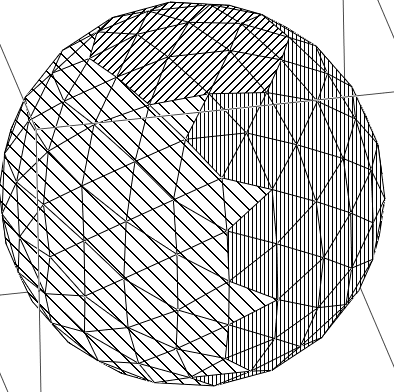
\includegraphics[scale=0.9]{zones.eps}
\end{center} 

\subsection*{Построение сетки}
Возьмем икосаэдр. Каждое ребро икосаэдра разделим пополам и
получившуюся точку спроектируем на сферу. С получившимся
многогранником можно проделать ту же самую процедуру. На каждом шаге
алгоритма шаг сетки уменьшается вдвое. 

\subsection*{Формулировка численной задачи}
Численная задача:
\begin{equation*}
\begin{split}
(\frac{1}{cos\psi}\frac{\partial}{\partial \phi} \phi_i, cos\phi
  \frac{\partial}{\partial \phi} \phi_j) 
+(\frac{1}{cos\psi}\frac{\partial}{\partial \lambda}\phi_i,
\frac{1}{cos\psi}\frac{\partial}{\partial \lambda}\phi_j ) = -(f,
\phi_j), \forall j, \forall i, \text{ для внутренних узлов } \\ 
u = u_0 \phi_i, \text { для граничных узлов, }
\end{split}
\end{equation*}
где $\phi_i$, $\phi_j$ - базисные функции.

Скалярное произведение:
\begin{equation*}
(u, v) = \int_\Omega u v ds = \int\int_\Omega u v cos(\phi)d\lambda d\phi.
\end{equation*}

Система уравнений:
\begin{equation*}
\sum_j x_j \sum_{k: \{j\in\bigtriangleup_k,
  i\in\bigtriangleup_k\}}\int_{\bigtriangleup_k}\frac{1}{cos\psi}(\frac{\partial}{\partial
  \phi} \phi_i) cos\phi (\frac{\partial}{\partial \phi}
\phi_j)+\frac{1}{cos^2\psi}\phi_i\phi_j ds =
\sum_{k:\{i\in\bigtriangleup_k\}}\int_{\bigtriangleup_k}f \phi_j ds, 
\end{equation*}
где
\begin{equation*}
u(\phi,\lambda)=\sum_i x_i \phi_i(\phi, \lambda),\\
f(\phi,\lambda)=\sum_i f_i \phi_i(\phi, \lambda).
\end{equation*}

При решении данной системы уравнений нужно будет считать интегралы вида:
\begin{equation*}
\begin{split}
\int_\bigtriangleup x^k y^n dx dy,\\
\int_\bigtriangleup x^k y^n cos(x) dx dy,\\
\int_\bigtriangleup x^k y^n / cos(x) dx dy.
\end{split}
\end{equation*}
Первый интеграл можно вычислить аналитически. Остальные два интеграла
можно считать так: вначале проинтегрировать по $y$, а потом использовать
квадратурную формулу для вычисления одномерного интеграла по $x$. Для
тестов использовалась квадратура Гаусса-Кронрода, использующая 15
узлов~\cite{kronrod}.

\subsection*{Численные результаты}
В качестве функции $u(\phi,\lambda)$ рассмотрим ограничение на сфере
функции:
\begin{equation*}
F(x,y,z)=0.5(x-1)^2+(y-z)^2+2(z-3)^2.
\end{equation*}
Данная функция взята, так как она не обладает симметричностью на
сфере. Правую часть для этой функции можно вычислить, например, в
свободнораспространяемом пакете {\it MAXIMA}~\cite{maxima}. Из-за громоздкости не
будем приводить вид правой части. 

В таблице приведена зависимость погрешности от размера сетки. В левом
столбце обозначено число итераций для алгоритма построения сетки. На
каждой итерации каждое ребро делится на два, поэтому шаг сетки
сокращается вдвое. При уменьшении шага в два раза погрешность
сокращается примерно в четыре раза.
\begin{center}
\begin{tabular}{| c | c | c | c |}
\hline
$It$ & число точек & погрешность \\
\hline
$1$ & $41$     & $2.73\times10^{+0}$ \\
$2$ & $161$    & $8.42\times10^{-1}$ \\
$3$ & $641$    & $2.73\times10^{-1}$ \\
$4$ & $2561$   & $7.09\times10^{-2}$ \\
$5$ & $10241$  & $2.06\times10^{-2}$ \\
$6$ & $40961$  & $5.80\times10^{-3}$ \\
$7$ & $163841$ & $1.61\times10^{-3}$ \\
\hline
\end{tabular}
\end{center}

Бибилиотека с реализацией алгоритма написана на языке $C++$,
сторонних библиотек не требуется. Скачать библиотеку и примеры её
использования, в том числе описанный пример решения уравнения лапласа на сфере можно с
сайта {\it http://www.resetius.ru}. (TODO: выложить всё)

\begin{thebibliography}{999}
\bibitem{bogach3} Богачев К. Ю., {\it  Практикум на ЭВМ.  Методы
    приближения функций, 3-е изд.}// M.:Изд-во
  механико-математического факультета МГУ. 2002.
\bibitem{maxima} Система компьютерной алгебры Maxima, {\it http://maxima.sourceforge.net/ru/}.
\bibitem{kronrod}Gauss–Kronrod quadrature formula, \\ {\it
  http://en.wikipedia.org/wiki/Gauss–Kronrod\_quadrature\_formula}. 
\end{thebibliography}

\end{document}

